\documentclass[10pt,twocolumn]{article}
\usepackage[margin=0.72in,columnsep=0.24in]{geometry}
\usepackage[T1]{fontenc}
\usepackage[utf8]{inputenc}
\usepackage{microtype}
\usepackage{graphicx}
\usepackage{booktabs}
\usepackage{array}
\usepackage{amsmath}
\usepackage{xcolor}
\usepackage{url}
\usepackage[hidelinks]{hyperref}
\usepackage{enumitem}
\usepackage{balance}
\setlist{nosep,leftmargin=*}
\setlength{\parskip}{2pt}
\setlength{\parindent}{1em}
\newcommand{\system}{\textsc{FunQA-Log}}
\newcommand{\code}[1]{\texttt{#1}}
\DeclareRobustCommand{\rawpath}[1]{\nolinkurl{#1}}
\newcommand{\yes}{\textcolor{green!45!black}{yes}}
\newcommand{\no}{\textcolor{red!65!black}{no}}

\title{Evidence-Bounded Local Retrieval-Augmented Generation for Game Logs:\\
A Vertical-Slice Case Study in Typed Failure Ownership}
\author{Anonymous submission}
\date{}

\begin{document}
\maketitle

\begin{abstract}
Retrieval-augmented generation (RAG) can expose source evidence, but retrieval alone does not make a generated claim correct, a failure attributable, or an execution path local.  We study a deliberately small game-log search vertical slice that treats these properties as independently testable contracts.  The system incrementally maps local JSONL records into PostgreSQL/pgvector with CocoIndex, retrieves a frozen evidence set, invokes a local Ollama model with a JSON Schema, and publishes a finding only after deterministic claim--evidence validation.  Every terminal state has an explicit owner---retrieval, synthesis, or none---and no alternate RAG stack is a permitted fallback.

We report a case study over nine synthetic records, eight indexed records, ten fixed queries, and one run for each of three Qwen2.5 model profiles (0.5B, 1.5B, and 3B), all recorded as Q4\_K\_M.  A standard-library extraction program independently replays the fixture assertions, rejects profile and hash inconsistencies, and derives all tables and figures from raw artifacts.  It reproduces 130/140, 130/140, and 136/140 passing assertions.  Only Q01 and Q03 exercise normal synthesis: both smaller profiles time out on both cases, while 3B publishes Q01 and rejects a schema-valid Q03 draft at the semantic gate.  Retrieval expectations remain unchanged across arms.  These observations are descriptive single-run evidence, not estimates of population performance.  The contribution is therefore not a claim that a model size ``wins,'' but an auditable method for separating retrieval correctness, wire-schema validity, semantic strictness, latency, and failure ownership in a local execution path.
\end{abstract}

\section{Introduction}
RAG combines a generator's parametric state with an explicit retrieved memory \cite{lewis2020rag}.  That separation is useful for mutable operational records, where a user should be able to inspect the log fragments behind a finding.  It is insufficient, however, to conclude that a generated claim is supported: a retriever may return the right records while generation times out, emits invalid structure, links the wrong record, or states a claim not entailed by the returned text.  Citation-oriented evaluation similarly distinguishes answer quality from citation completeness and correctness \cite{gao2023alce}.

This paper asks a narrower systems question: \emph{can a local game-log RAG slice make each boundary observable and assign failures without silently crossing the evidence boundary?}  The target is not open-domain question answering or production-scale search.  It is an evidence-bounded path for a fixed game-operations corpus in which retrieval, synthesis, freshness, typed failure states, and provenance can be inspected separately.

\system{} follows one path: JSONL records, CocoIndex state, PostgreSQL/pgvector retrieval, local Ollama synthesis, a FastAPI stream, and a same-origin web proxy.  The design excludes the application's existing Genkit path, cached answers, model-prior answers, and non-CocoIndex evidence as fallbacks.  The key systems choice is to make an unsuccessful stage a first-class result rather than an invitation to switch owners.  A retrieval outage therefore remains \code{retrieval\_unavailable}; a post-retrieval model outage remains \code{synthesis\_unavailable} while preserving the evidence already found; a schema-valid but semantically unsupported draft becomes \code{weak\_support} and publishes no finding.

The evaluation is intentionally bounded.  The frozen corpus contains nine synthetic records, of which eight are indexed; the query manifest contains ten cases.  Only Q01 and Q03 traverse normal synthesis.  Each of three exact model profiles has one ten-query run.  These facts are emitted in \rawpath{results/run_summary.csv}; the shared corpus and query hashes and each raw run directory appear in the same rows.  Consequently, we use raw observations and descriptive comparisons only: no confidence interval, $p$-value, percentile, or significance test is meaningful here.

This paper makes three contributions:
\begin{enumerate}
  \item We specify an evidence-bounded orchestration pattern that separates retrieval correctness, response-schema validity, deterministic semantic support, freshness, latency, and owner-aware failure states.
  \item We provide an auditable, standard-library artifact builder that verifies common corpus/query hashes, exact model profiles, Q4\_K\_M quantization, stream identity, provenance membership, and independently recomputed assertions before generating tables and vector figures.
  \item We report a nine-record, ten-query vertical-slice case study and an isolated incremental-dataflow observation.  The study exposes both positive behavior (stable retrieval and one strictly accepted 3B finding) and negative behavior (four synthesis timeouts and one semantic rejection) without converting failures into model answers.
\end{enumerate}

\section{Related Work}
\subsection{Retrieval and adaptive correction}
Foundational RAG retrieves non-parametric memory for generation and reports gains on the evaluated Wikipedia-backed tasks \cite{lewis2020rag}; it does not establish source faithfulness for local game logs.  FLARE performs active retrieval during generation when predicted text contains low-confidence tokens \cite{jiang2023flare}.  Self-RAG trains reflection tokens to decide when to retrieve and to critique relevance, support, and utility \cite{asai2024selfrag}.  CRAG evaluates retrieved evidence and applies corrective actions, including a web-search path \cite{yan2024crag}.  These methods motivate conditional retrieval and correction, but their training regimes, corpora, and external-source assumptions differ from our fixed local evidence boundary.  In particular, CRAG's web extension is out of contract here.

Our orchestrator does not learn when to retrieve and does not repeatedly query during generation.  It instead freezes one returned set, exposes its hash, and either accepts the generated claims against that set or declines to publish them.  This is a systems-control contribution rather than a new retrieval or language-model algorithm.

\subsection{RAG evaluation and structured generation}
RAGAs decomposes evaluation into faithfulness, answer relevance, and context relevance \cite{es2024ragas}.  ARES uses synthetic data, trained judges, and a human-labeled calibration set to evaluate context relevance, faithfulness, and answer relevance \cite{saadfalcon2024ares}.  These frameworks are valuable at larger study scale, but neither is annotation-free ground truth for this bilingual-capable, synthetic game-log fixture.  We therefore use the frozen query oracle and deterministic predicates rather than an LLM judge.

Grammar-constrained decoding can guarantee conformity to a formal structure for the evaluated structured NLP tasks \cite{geng2023grammar}; Ollama documents a JSON-Schema \code{format} interface and recommends validating returned content client-side \cite{ollama2026structured}.  Structural conformity does not imply factual support.  Our measurement consequently records terminal wire validity, synthesis-schema status, and semantic strictness as separate fields.

\subsection{Incremental and local data systems}
CocoIndex documents a declarative state-to-target execution model and memoized per-item processing \cite{cocoindex2026core}.  Differential Dataflow provides a research analogue for propagating changes through declarative computations while reusing prior state \cite{mcsherry2013differential}; we do not claim that CocoIndex implements Differential Dataflow.  pgvector supplies exact nearest-neighbor search by default and optional approximate indexes such as HNSW \cite{pgvector2026,malkov2020hnsw}.  Sentence-BERT established efficient independent sentence embeddings for cosine comparison \cite{reimers2019sbert}; the current Sentence Transformers API exposes that usage \cite{sentenceTransformers2026sts}.  None of these sources transfers accuracy or latency numbers to this corpus.

Local and edge RAG systems have explored mobile memory, latency, and online-index tradeoffs \cite{park2025mobilerag,seemakhupt2024edgerag}.  Their author-reported preprint results concern different devices and index architectures.  Here, ``local'' denotes the configured execution boundary---local files, PostgreSQL, and a loopback Ollama endpoint in the captured runs---not a privacy, security, energy, or deployment guarantee.

\section{System Design}
\subsection{One evidence path}
The frozen architecture contract defines the following path:
\begin{center}
\small
JSONL $\rightarrow$ CocoIndex $\rightarrow$ PostgreSQL/pgvector\\
$\rightarrow$ retrieval $\rightarrow$ local Ollama $\rightarrow$ typed stream.
\end{center}
CocoIndex discovers local JSONL files.  A memoized per-file function validates one record, excludes the designated freshness fixture, computes the excerpt hash, embeds the excerpt, and declares a row keyed by evidence ID.  The target contains provenance fields alongside the vector.  SQL retrieval filters by snapshot, time, source, project, and entity, then orders by cosine distance with deterministic time and evidence-ID tie breakers.  The score is $1-\text{distance}$ and is never relabeled as a probability.

The returned evidence snapshot is immutable within a dispatch.  Each item repeats the query and correlation identities, source and snapshot identifiers, excerpt offsets, trust class, and content hash.  A SHA-256 digest over ordered evidence-ID/hash pairs names the set.  The artifact builder rejects evidence outside the eight-ID index manifest, malformed content hashes, or identity/snapshot drift.

\subsection{Ordered orchestration and typed ownership}
A dispatch emits an acceptance frame, retrieval and ranking stages, zero or one evidence snapshot, an optional synthesis stage, and exactly one terminal or cancelled frame.  Freshness is checked before synthesis.  Empty evidence maps to \code{no\_hits}; a request beyond snapshot coverage maps to \code{stale\_index}; deterministic insufficient-evidence cases map to \code{weak\_support}.  The terminal mapping fixes outcome, owner, confidence label, and recovery action together, as summarized in Table~\ref{tab:ownership}.

\begin{table}[t]
\centering
\caption{Terminal ownership is a type-level contract, not a post-hoc label.}
\label{tab:ownership}
\small
\begin{tabular}{@{}lll@{}}
\toprule
Outcome & Owner & Published finding \\
\midrule
\code{supported} & none & strict finding \\
\code{no\_hits} & none & none \\
\code{weak\_support} & none & none \\
\code{stale\_index} & retrieval & none \\
\code{retrieval\_unavailable} & retrieval & none \\
\code{synthesis\_unavailable} & synthesis & none \\
\bottomrule
\end{tabular}
\end{table}

This mapping prevents category collapse.  For example, a model timeout after retrieval does not invalidate already returned evidence and does not become a retrieval failure.  Conversely, a retrieval fault cannot be hidden by calling another generator.  Cancellation is outside the six terminal outcomes and preserves any evidence already emitted.

\subsection{Schema constraint and semantic gate}
The local synthesizer receives the query, visible scope, and only the frozen returned evidence.  The system prompt treats excerpts as data, denies tools and alternate sources, and requests three top-level objects: a summary, material claims, and claim-to-evidence links.  Ollama receives the Pydantic-derived JSON Schema as its \code{format}; temperature is zero.  The service then parses JSON and validates the draft against that schema.

A second, deterministic gate operates after schema validation.  Claim IDs must be contiguous; every link must target returned evidence; untrusted evidence must use the \code{untrusted\_data} relation; every material claim must have returned \code{supports} evidence with lexical overlap; impossible numeric direction is rejected; and coverage must be complete.  Correction semantics are generic: evidence labeled \code{supersedes} must also support the claim, while the same claim must link prior context or contradiction.  The production gate contains no P42, incident-184, or E001/E004/E006/E009 branch; fixture-specific expected values and IDs remain in the runner oracle.  A schema-valid draft that fails any semantic predicate produces \code{weak\_support} and no finding.  JSON parse or schema failure instead produces \code{synthesis\_unavailable} with reason \code{malformed\_synthesis}.  A timeout remains a timeout; it is not counted as either schema-valid or schema-invalid because no draft was observed.

\subsection{Incremental flow}
The index function is memoized per file and mounted over a live local-file source.  The isolated evidence packet contains a baseline, a no-op execution, and a one-change execution.  These artifacts are not interleaved with the model runs and their modified E001 row is not compared to the frozen query-run row.  This separation avoids treating a dataflow smoke test as an end-to-end retrieval benchmark.

\section{Threat Model}
The protected properties are evidence membership, provenance identity, owner-correct terminal states, and refusal to publish unsupported claims.  Trusted components are the checked-out code, fixture manifests, local database, configured Ollama endpoint, and host operating environment for the observed runs.  The corpus itself can contain untrusted text: E009 is an injection canary and is typed \code{untrusted\_data}.  Component outages, timeouts, malformed model output, stale snapshots, wrong evidence links, and unsupported claims are in scope.

The design mitigates these threats by constraining inputs, retaining content and set hashes, using parameterized SQL, prohibiting model tools, validating schemas client-side, checking all evidence links against the frozen set, and mapping failures to owners.  The fixture runner also records requests made by its own \code{httpx} client and scans serialized streams for the canary and non-index IDs.

Several threats are explicitly out of scope.  A compromised host, database, Ollama binary, model weights, or artifact builder can falsify local evidence.  The runner hook does not observe unrelated browser or operating-system traffic.  It has no packet capture, HAR, remote attestation, side-channel analysis, or authorization audit.  Two reported canary fields---cached-answer use and prior-knowledge answers---are constants in the runner rather than independent detectors.  Therefore the negative control supports only the instrumented runner path; it does not prove global network isolation, privacy, confidentiality, or absence of model memorization.

\section{Experimental Protocol}
\subsection{Frozen inputs and arms}
The fixture corpus is \code{sim-game-logs-v1}: nine JSONL records, with E001--E006 and E008--E009 indexed and E007 intentionally excluded.  The index snapshot is \code{sim-index-v1}.  The corpus SHA-256 is
\begin{quote}\tiny\ttfamily
\detokenize{ddf326aa636543a4c77dcf1262bd55e2b388ef1cae709f75f9a6b66f1d8f9ad2}.
\end{quote}
The ten-query manifest SHA-256 is
\begin{quote}\tiny\ttfamily
\detokenize{5fe747e2cf2c8f52cafc2468426e00f41295dfefe9eacbf66091369df35eed33}.
\end{quote}
Both values, record/query counts, and each raw directory are emitted in \rawpath{results/run_summary.csv}.

The compared synthesis profiles are exactly \code{qwen2.5:0.5b}, \code{qwen2.5:1.5b}, and \code{qwen2.5:3b}.  Each fixture manifest, environment allowlist, and synthesis terminal records \code{Q4\_K\_M}.  Other common fields---CocoIndex version, embedding model, ranking seed, clock, snapshot membership, build ID, and hashes---must match byte-for-byte or structurally before the script writes results.  There is one ten-query run per arm.  Hardware metadata was not emitted in these raw artifacts and remains unreported.
The raw model runs predate the generic semantic-gate change described in Section~3.3.  Their quantitative rows remain a historical observation of the frozen run artifacts; the builder re-derives assertions from those artifacts and does not re-execute the current synthesizer.  Consequently, the model-arm results below must not be interpreted as an evaluation of the generalized gate.

\subsection{Queries and controls}
Q01 asks for an exact cooldown change and rationale; Q03 asks for an incident cause and fix while preserving a retraction/correction relationship.  These are the only normal synthesis-dependent cases.  Q02, Q08, and Q09 are deterministic weak-support boundaries; Q04 is no-hit; Q05 and Q10 inject retrieval unavailability; Q06 injects synthesis unavailability after retrieval; and Q07 requests coverage beyond the frozen snapshot.  The all-ten aggregate is therefore dominated by deterministic boundary and fault behavior and is not a model-quality score.

Q10 is the no-fallback negative control.  We report the five fields written by each \code{canary-scan.txt}, but distinguish the three observed scans (runner-hook Genkit URLs, canary occurrences, non-index evidence IDs) from the two runner constants (cache and prior-knowledge counters).

The CocoIndex experiment is a separate three-step execution over nine files: baseline, no-op, and one-change.  Its console statistics and displayed elapsed values are parsed from four text artifacts.  The experiment has no repetitions and is used to check change selectivity, not to estimate throughput.

\subsection{Derived metrics and rejection rules}
The builder reconstructs each of fourteen assertions per query from streams and the frozen oracle: outcome, owner, query/correlation identity, minimum evidence count, required top-five IDs, expected rank one, forbidden values, required finding values, scope, scope delta, snapshot, boundary reason, and recovery action.  It then requires exact agreement with the raw \code{results.json} rows.  It separately checks the terminal wire shape and strict supported-finding invariants.

For Q01/Q03, synthesis schema status is \emph{valid} when a structured draft reaches semantic validation, \emph{invalid} only for \code{malformed\_synthesis}, and \emph{not observed} when synthesis fails before a draft is available.  Semantic rejection is counted only for a schema-valid draft that produces \code{weak\_support}.  This prevents a timeout from being mislabeled as a schema defect.

Latency is the runner's per-case monotonic duration from \code{correlated-spans.json}.  The fixture constructs a new sentence-transformer embedder for each case, so the duration includes setup/cache effects and cannot isolate retrieval from synthesis.  We show raw Q01/Q03 observations and no percentiles.  The full-run duration is retained in the CSV but is not used as query latency.

\section{Results}
\subsection{Contract outcomes}
Table~\ref{tab:run-summary} and Figure~\ref{fig:assertions} report the independently reconstructed assertions.  The 0.5B and 1.5B runs each pass 130/140; the 3B run passes 136/140.  All three raw runner exit codes are 1 because at least one assertion fails.  Exact-outcome accuracy is 8/10, 8/10, and 9/10, respectively.  These counts are rows in \rawpath{results/run_summary.csv}; all 420 individual comparisons, including expected and observed JSON values, are in \rawpath{results/assertions.csv}.

\begin{table}[t]
\centering
\caption{Single-run descriptive results.  ``Strict'' is supported Q01/Q03.  ``Syn. schema'' is valid/invalid/unobserved over those two cases.}
\label{tab:run-summary}
\small
\begin{tabular}{@{}lrrrr@{}}
\toprule
Profile & Assert. & Outcome & Strict & Syn. schema \\
\midrule
0.5B & 130/140 & 8/10 & 0/2 & 0/0/2 \\
1.5B & 130/140 & 8/10 & 0/2 & 0/0/2 \\
3B   & 136/140 & 9/10 & 1/2 & 2/0/0 \\
\bottomrule
\end{tabular}
\end{table}

\begin{figure}[t]
\centering
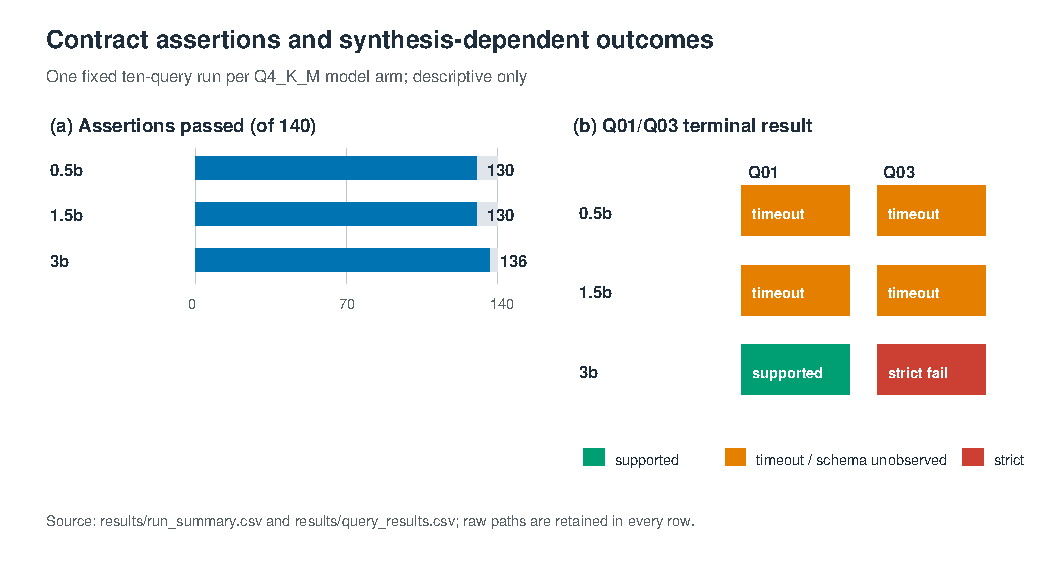
\includegraphics[width=\columnwidth]{figures/assertions-and-semantics.pdf}
\caption{The aggregate assertion difference is explained by two synthesis-dependent cases, not by a broad ten-query model-quality comparison.  Source: \rawpath{results/run_summary.csv} and \rawpath{results/query_results.csv}.}
\label{fig:assertions}
\end{figure}

The terminal wire-schema validator reports zero failures in each arm.  This statement concerns terminal envelope invariants, not the model draft.  On Q01/Q03, the smaller profiles produce four timeouts in total, so schema validity is unobserved for those four attempts.  The 3B arm returns two schema-valid drafts: Q01 passes the semantic gate, while Q03 is rejected by strict support.  No observed Q01/Q03 attempt is classified as malformed synthesis.  Thus ``zero schema-invalid drafts'' must not be read as ``all drafts were schema-valid''; four drafts never arrived.

\subsection{Retrieval invariants}
All three arms retrieve the same ordered evidence IDs for each query that has evidence.  Q01 returns E001, E002, E003; Q03 returns E004, E006, E005, preserving the correction directly after the initial hypothesis; Q08 returns only the untrusted E009.  Across each arm, the frozen required-ID numerator is 9/9 at rank five, and all ten \code{required\_top\_five} assertions pass.  The runner's ten \code{expected\_rank\_one} assertions also pass per arm, although only four cases define a non-null expected rank-one ID.  Per-case numerators, denominators, ordered IDs, exact-ID ranks, raw stream paths, and snapshot IDs are in \rawpath{results/retrieval_by_query.csv}.

These observations establish contract conformance on this fixture, not general retrieval quality.  The corpus and queries were co-designed, the retrieval implementation includes explicit E004/E006 adjacency, and there are no graded judgments for nDCG.  We therefore do not report nDCG or transfer any SBERT/pgvector benchmark result.

\subsection{Synthesis-dependent cases and latency}
Table~\ref{tab:synthesis} shows Q01 and Q03.  The 0.5B arm times out after 33.426~s on Q01 and 23.918~s on Q03.  The 1.5B arm times out after 26.754~s and 11.695~s.  The 3B arm supports Q01 after 18.465~s and returns a schema-valid but semantically rejected Q03 draft after 19.355~s.  Values are rounded renderings of the millisecond rows in \rawpath{results/query_results.csv}; Figure~\ref{fig:latency} plots the same rows without error bars.

\begin{table}[t]
\centering
\caption{Observed Q01/Q03 terminal results and whole-case latency.  One observation exists per cell.}
\label{tab:synthesis}
\small
\begin{tabular}{@{}llll@{}}
\toprule
Profile & Case & Outcome & Seconds \\
\midrule
0.5B & Q01 & synthesis timeout & 33.426 \\
0.5B & Q03 & synthesis timeout & 23.918 \\
1.5B & Q01 & synthesis timeout & 26.754 \\
1.5B & Q03 & synthesis timeout & 11.695 \\
3B   & Q01 & supported & 18.465 \\
3B   & Q03 & strict weak support & 19.355 \\
\bottomrule
\end{tabular}
\end{table}

\begin{figure}[t]
\centering
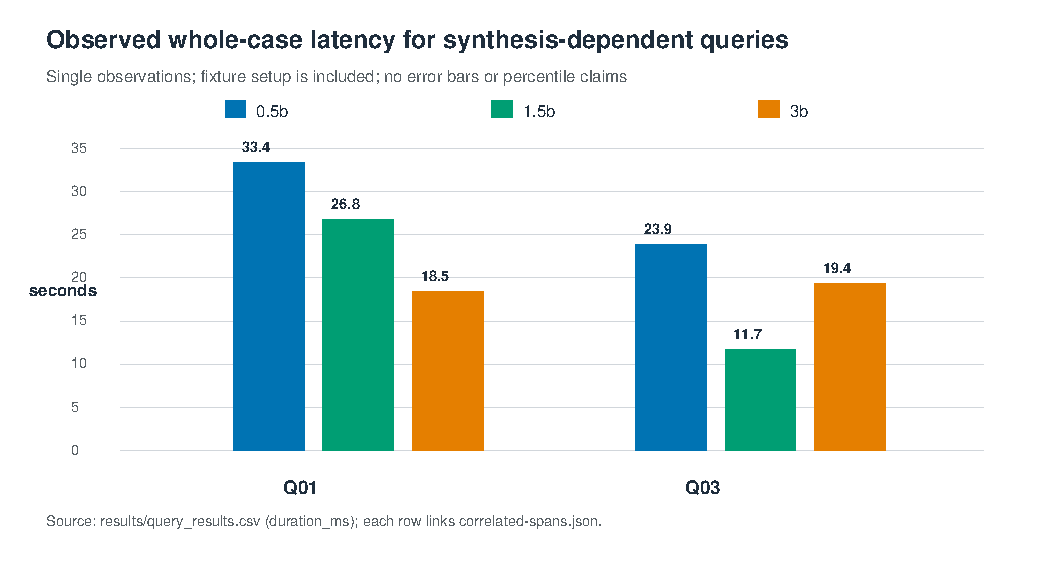
\includegraphics[width=\columnwidth]{figures/latency-q01-q03.pdf}
\caption{Raw whole-case latency for the two normal synthesis cases.  Setup and cache effects are included, and there is one observation per profile/case.  Source: \rawpath{results/query_results.csv}.}
\label{fig:latency}
\end{figure}

The data do not support a monotonic latency claim: Q03 is faster for 1.5B than 3B in these single observations, while Q01 decreases with profile size.  Nor do they support a general quality ranking.  The only defensible descriptive statement is that 3B is the sole arm to publish a strict finding, on Q01, in this run; all models fail the Q03 expected outcome, for different reasons.

\subsection{No-fallback negative control}
For each arm, \code{canary-scan.txt} reports zero runner-hook Genkit network spans, zero canary occurrences, and zero non-CocoIndex evidence IDs.  Q10 remains a typed retrieval-owned unavailable result in \rawpath{results/query_results.csv}.  The same files report zero cached-answer and prior-knowledge use, but the implementation initializes those two counters to zero; they are not active monitors.  All five fields and their instrumentation scope are retained in \rawpath{results/canary_summary.csv}.  We therefore describe this as a negative observation for the instrumented fixture path, not proof of system-wide no-fallback behavior.

\subsection{Incremental dataflow}
Figure~\ref{fig:incremental} and Table~\ref{tab:incremental} show the isolated CocoIndex experiment.  Baseline reports nine added files; the no-op reports nine unchanged; one-change reports one reprocessed and eight unchanged.  The displayed elapsed observations are 12.5, 0.0, and 11.4~s.  They are single console observations and not a benchmark.  The useful result is selectivity: the no-op and one-change statistics distinguish unchanged from reprocessed per-file work.  \rawpath{results/cocoindex_incremental.csv} retains each source text path; \rawpath{results/cocoindex_target_row.csv} retains the post-change E001 row and hash.

\begin{table}[t]
\centering
\caption{Isolated incremental-flow observations over nine files.}
\label{tab:incremental}
\small
\begin{tabular}{@{}lrrrr@{}}
\toprule
Phase & Added & Reproc. & Unchanged & Shown s \\
\midrule
baseline & 9 & 0 & 0 & 12.5 \\
no-op & 0 & 0 & 9 & 0.0 \\
one-change & 0 & 1 & 8 & 11.4 \\
\bottomrule
\end{tabular}
\end{table}

\begin{figure}[t]
\centering
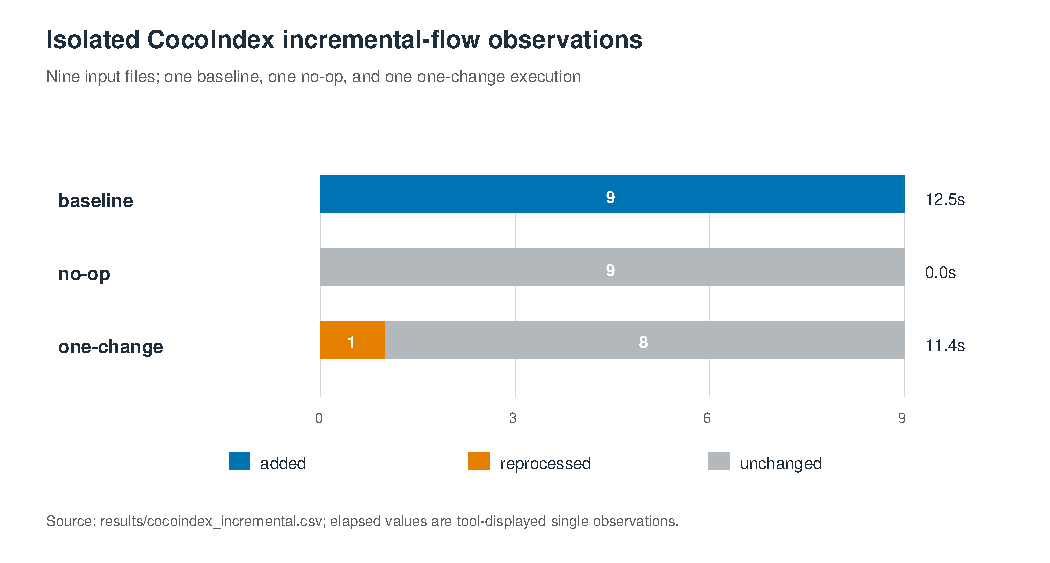
\includegraphics[width=\columnwidth]{figures/incremental-dataflow.pdf}
\caption{CocoIndex console classifications for baseline, no-op, and one-change executions.  Source: \rawpath{results/cocoindex_incremental.csv}.}
\label{fig:incremental}
\end{figure}

\section{Failure Analysis}
\paragraph{Timeout dominates the smaller arms.}
Q01 and Q03 each lose five assertions in the 0.5B and 1.5B runs: expected outcome, owner, required finding values, boundary reason, and recovery action.  Retrieval assertions still pass.  The observed terminal is synthesis-owned \code{synthesis\_unavailable} with \code{synthesis\_timeout}; no draft exists to classify structurally or semantically.  The orchestrator therefore preserves evidence and chooses \code{open\_raw\_evidence}, as designed, while the fixture oracle expected a supported finding and \code{inspect\_claim\_traces}.

\paragraph{3B Q03 is a semantic, not structural, failure.}
The 3B Q03 attempt reaches the JSON/schema parser and records model token counts, but the deterministic validator returns no finding.  The terminal is \code{weak\_support} with owner \code{none}.  Four oracle assertions fail: outcome, required finding values, boundary reason, and recovery action.  Owner correctness does not fail because both the expected supported state and observed weak-support state are non-failure outcomes owned by \code{none}.  This distinction is visible only because schema validity and semantic strictness are separate columns.

\paragraph{Aggregate counts conceal causal structure.}
The 136/140 figure for 3B looks close to the 130/140 figures for smaller models, but the six-assertion difference combines one successful Q01 transition with a differently typed Q03 failure.  Eight other cases are deterministic or fault-driven and contribute no normal synthesis-quality comparison.  Reporting only the aggregate would therefore overstate both coverage and model evidence.

\paragraph{Failure ownership remains useful when correctness fails.}
The unsuccessful runner exit codes are not a systems collapse.  In the smaller arms, synthesis timeouts are correctly owned and evidence remains inspectable.  In 3B Q03, semantic insufficiency is represented without assigning a component outage.  Typed failure ownership does not make the answer correct; it makes the failure diagnosable and prevents an alternate source from masquerading as recovery.

\section{Limitations and Ethics}
\paragraph{External validity.}
This is a vertical-slice case study with nine synthetic records, eight indexed records, ten hand-authored English queries, one run per profile, and only two normal synthesis cases.  It cannot establish production-scale throughput, open-domain retrieval quality, robustness across games, bilingual retrieval effectiveness, user utility, or general model-size trends.  The embedding model can process multilingual text, but no Korean query fixture is present.

\paragraph{Statistical validity.}
There are no repetitions.  We report no confidence intervals, $p$-values, standard errors, percentiles, or significance claims.  Query durations include per-case embedder construction and unknown cache/thermal effects.  Hardware, operating-system, Ollama-version, model digest, CPU/GPU time, and peak memory were not emitted by these artifacts.  Parameter count and latency are therefore confounded with uncontrolled run conditions.

\paragraph{Construct validity.}
The fixed query oracle checks contract conformance, not unconstrained factuality.  Q01/Q03 expected values remain fixture-runner assertions, while the current production semantic gate uses generic returned-evidence coverage, relation, lexical-overlap, numeric-direction, and correction rules.  The frozen runs predate that generalization, so they do not measure its effect.  Q03 retrieval still explicitly places a correction next to the initial hypothesis.  Schema validity only states that a draft reached semantic validation; the conservative semantic predicates are not entailment proofs, and rejection can discard a useful answer.  No human evaluation was conducted.

\paragraph{No-fallback and privacy boundaries.}
The runner observes its own \code{httpx} requests and serialized streams.  It does not observe the full browser, server process tree, or operating system.  Two scan fields are constants.  ``Local execution'' names the configured path, not a verified privacy guarantee.  The artifact includes synthetic log excerpts and stable fixture identifiers; using the design with real operational logs would require access control, retention, redaction, audit, and incident-response analysis not evaluated here.

\paragraph{Responsible claims.}
A failed synthesis is not rescued by model prior knowledge.  This reduces the chance of presenting untraceable content, but it can reduce availability.  Users must be shown evidence and boundary reasons, not only a supported/unsupported badge.  The study makes no claim of acceptance readiness, production deployment, security certification, or replacement of human incident judgment.

\section{Artifact Availability}
All manuscript artifacts live under \rawpath{study/genai-game-log-rag/}.  From the repository root, regenerate results and figures with:
\begin{quote}\small
\rawpath{python3 study/genai-game-log-rag/scripts/build_results.py}
\end{quote}
The script uses only the Python standard library.  It exits with status 2 before writing if the evidence contract is inconsistent.  CSV and figure manifests record SHA-256 digests of generated outputs.

Compile the anonymous two-column paper from its directory with:
\begin{quote}\small\ttfamily
pdflatex -interaction=nonstopmode -halt-on-error paper.tex\\
bibtex paper\\
pdflatex -interaction=nonstopmode -halt-on-error paper.tex\\
pdflatex -interaction=nonstopmode -halt-on-error paper.tex
\end{quote}
\rawpath{REPRODUCIBILITY.md} lists the same commands, artifact map, dependency boundary, and expected extraction summary.

\section{Conclusion}
An evidence path is more useful when its failure modes are as explicit as its successful findings.  \system{} combines incremental local indexing, deterministic retrieval provenance, constrained local synthesis, strict claim--evidence validation, and typed ownership without an alternate fallback.  In this limited case study, retrieval contracts remain stable while synthesis behavior differs: two smaller profiles time out on both normal synthesis cases, and 3B accepts one case while rejecting the other semantically.  The result is not a general ranking of Qwen models.  It is a reproducible demonstration that schema validity, semantic support, latency, and owner-correct failure can be measured separately rather than compressed into one RAG score.

\appendix
\section{Raw Artifact Map}
The authoritative model-run directories are:
\begin{itemize}
  \item \rawpath{_workspace/current/qa/evidence/stage-1/fixture-run-qwen0_5b-schema/}
  \item \rawpath{_workspace/current/qa/evidence/stage-1/fixture-run-qwen1_5b/}
  \item \rawpath{_workspace/current/qa/evidence/stage-1/fixture-run-qwen3b/}
\end{itemize}
Each contains \code{fixture-manifest.json}, \code{index-manifest.json}, \code{queries.json}, \code{results.json}, \code{streams.json}, \code{correlated-spans.json}, \code{canary-scan.txt}, copied hash files, command/environment records, timestamps, duration, exit code, stdout, and stderr.

The isolated incremental artifacts are:
\begin{itemize}
  \item \rawpath{_workspace/current/engineering/evidence/stage-1/cocoindex-experiment-baseline.txt}
  \item \rawpath{_workspace/current/engineering/evidence/stage-1/cocoindex-experiment-noop.txt}
  \item \rawpath{_workspace/current/engineering/evidence/stage-1/cocoindex-experiment-one-change.txt}
  \item \rawpath{_workspace/current/engineering/evidence/stage-1/cocoindex-experiment-target-row.txt}
\end{itemize}

\section{Derived Artifact Schema}
\rawpath{results/run_summary.csv} is one row per model arm.  \rawpath{results/query_results.csv} is one row per model/query pair and contains identities, expected and observed states, duration, ordered evidence IDs, schema/semantic status, token fields, and raw paths.  \rawpath{results/assertions.csv} contains all independently reconstructed assertions.  \rawpath{results/retrieval_by_query.csv} contains retrieval numerators, denominators, ranks, and raw stream paths.  \rawpath{results/canary_summary.csv} states instrumentation scope.  The two CocoIndex CSV files preserve execution classes and the isolated post-change target row.

\section{Rejection Tests}
Before aggregation, the builder requires: exact profile-to-directory mapping; Q4\_K\_M in both manifest and environment; identical common profile fields; query bytes matching the query hash; the current corpus matching the corpus hash; ten unique cases; ten spans; fourteen known assertions per case; independently reconstructed assertions equal to raw rows; terminal identities equal to query identities; evidence IDs inside the index manifest; lowercase 64-hex content hashes; snapshot consistency; finding links confined to returned evidence; and exit code consistent with assertion failure.  These checks make a copied or edited artifact fail closed rather than silently entering a figure.

\balance
\bibliographystyle{plain}
\bibliography{references}
\end{document}
